\section{Generative Model}

\subsection{Diffusion Model}
\subsubsection{Diffusion}
\paragraph{DDPM}
DDPM is like splitting the encoder and decoder of VAE into controllable parts. 
For each training data point $x_0\sim p_{data}$, then a discrete Markov chain $\{x_1, \cdots, x_N\}$ is constructed by transition function:
\begin{equation}
    p(x_i|x_{i-1})=\mathcal{N}(x_i|\sqrt{1-\beta_i}x_{i-1}, \beta_i I)
\end{equation}
Then we can get 
\begin{equation}
    p_{\alpha_i}(x_i|x_0) = \mathcal{N}(x_i|\sqrt{\alpha_i}x_0, (1-\alpha_i)I), \alpha_i = \Pi_{j=1}^i(1-\beta_j)
\end{equation}
So, when $\alpha_i\to 0$, $p_{\alpha_i}(x_i|x_0)$ is close to $N(0, I)$. For generating  new data samples, DDPMs start by first generating an unstructured noise vector from the prior distribution (which is  typically trivial to obtain), then gradually remove noise therein by running a learnable Markov chain in the reverse  time direction.
The reverse is to learn transition kernel $p_\theta(x_{i-1}|x_i)$ having form:
\begin{equation}
    p_\theta(x_{i-1}|x_i) = \mathcal{N}(x_{i-1}|\mu_\theta(x_i, i), \Sigma_\theta(x_i, i))
\end{equation}
where $\theta$ denotes model parameters. Key to the success of this sampling process is training the reverse Markov chain to match the actual time reversal  of the forward Markov chain.
That is, $p_\theta(x_0, x_1, \cdots, x_N)p(x_N)\Pi_{i=1}^Np_\theta(x_{i-1}|x_i)$ should be close to $q(x_0, x_1, \cdots, x_N)=p(x_0)\Pi_{i=1}^Np_{\alpha_i}(x_i|x_{i-1})$.
This is achieved by minimizing the KL divergence between these two:
\begin{equation}
    \begin{aligned}
        &KL(q(x_0, x_1, \cdots, x_N)||p_\theta(x_0, x_1, \cdots, x_N))\\
        =&-\mathbf{E}_{q}\left[\log p_\theta(x_0, x_1, \cdots, x_N)\right] + const\\
        =&-\mathbf{E}_{q}\left[\log p(x_N) + \sum_{i=1}^N \log \frac{p_\theta(x_{i-1}|x_i)}{q(x_i|x_{i-1})}\right]
    \end{aligned}
\end{equation}

% Hence we need to train the ELBO:
% \begin{equation}
%     \operatorname{ELBO}(x) = \sum_{i=1}^N(1-\alpha_i)\mathbf{E}_{p_{data}(x)}\left[\mathbf{E}_{p_{\alpha_i}(\hat{x}|x)}\left[\|s_\theta(\hat{x}, i) - \nabla_{\hat{x}}\log p_{\alpha_i}(\hat{x}|x)\|\right]\right]
% \end{equation}
% Then do the reverse Markov chain.

This is clearly a discrete version. Then we consider the continuous version.
\paragraph{Score SDEs}
We consider linear SDE having the form:
\begin{equation}
    dX_t = (a(t)X_t + b(t))dt + g(t)dW_t
\end{equation}
where $X_t\in \mathcal{R}^d, W_t\in \mathcal{R}^m$ with diffusion factor $Q\in \mathcal{R}^{m\times m}$, then $a(t)\in \mathcal{R}^{d\times d}, b(t)\in \mathcal{R}^d, g(t)\in \mathcal{R}^{d\times m}$. 
By Euler Maruyama method, it can be approximated By
\begin{equation}
    \begin{aligned}
        X_{t+s}&=X_t + (a(t)X_t + b(t))s+g(t)\sqrt{sQ}\xi\\
        &=(1+a(t)s)X_t + b(t)s + g(t)\sqrt{sQ}\xi
    \end{aligned}
\end{equation}
where $\xi\sim N(0, I_m)$. Usually we need to consider the expectation, variance and distribution of $X_t$. But the stochastic value of $X_t$ is dependent of $x_0$. Then first we consider
\begin{equation}
    \begin{aligned}
    E\left[X_{t+s} | X_{0}\right]-E\left[X_{t} | X_{0}\right] & \approx\left(a(t) E\left[X_{t} | X_{t}\right]+b(t)\right) s+g(t) \sqrt{sQ} E[\xi] \\
    & =\left(a(t) E\left[X_{t} | X_{0}\right]+b(t)\right) s .
    \end{aligned}
\end{equation}


Note  $e(t)=E\left[X_{t} | X_{0}\right]$, then
\begin{equation}
    e^{\prime}(t)=\lim _{s \rightarrow 0} \frac{E\left[X_{t+s} | X_{0}\right]-E\left[X_{t} | X_{0}\right]}{s}=a(t) \cdot e(t)+b(t) . \quad e(0)=X_{0} .    
\end{equation}
which is an ODE system, having solution
\begin{equation}
    e(t)=e^{\int_{0}^{t} a(s) d s}\cdot\left(X_{0}+\int_{0}^{t} e^{-\int_{0}^{s} a(r) d r} b(s) d s\right)
\end{equation}
Therefore
\begin{equation}
    \begin{aligned}
    E\left[X_{t}\right] & =E\left[E\left[X_{t} | X_{0}\right]\right]=E[e(t)] \\
    & =e^{\int_{0}^{t} a(s) d s}\cdot\left(E\left[X_{0}\right]+\int_{0}^{t} e^{-\int_{0}^{s} a(r) d r} b(s) d s\right) 
    \end{aligned}
\end{equation}

Similarly, Note $\operatorname{Var}\left(X_{0} | X_{0}\right)=v(t)$:
then $\operatorname{Var}\left(X_{t+s} | X_{0}\right)=(1+s a(t))^{2} \operatorname{Var}\left(X_{t} | X_{0}\right)+s gQg^\top$. Then
\begin{equation}
    \begin{aligned}
        V^{\prime}(t)&=\lim _{s \rightarrow 0} \frac{\operatorname{Var}\left(X_{t+s} | X_{0}\right)-\operatorname{Var}\left(X_{t} | X_{0}\right)}{s}\\
        =&\left[\left(a^{2}(t) s+2 a(t)\right) v(t)+g^{2}(t)\right]|_{s \rightarrow 0}\\ 
        =&2 \alpha(t) V(t)+g(t)Qg^\top(t), \qquad V(0)=0
    \end{aligned}
\end{equation}
Solution is:
\begin{equation}
    v(t)=e^{\int_{0}^{t} 2a(s) d s}\cdot\left(\int_{0}^{t} e^{-\int_{0}^{s} 2 a(r) d r} g(s)Qg^\top(s) d s\right)
\end{equation} 
By law of total variance:
\begin{equation}
    \begin{aligned}
        \operatorname{Var}\left(X_{t}\right)=&E\left[X_{t}^{2}\right]-E^{2}\left[X_{t}\right]=E\left[ E\left[X_{t}^{2} | X_{0}\right]\right]-E^{2}\left[X_{t}\right] \\
        =&E\left[\operatorname{Var}\left(X_{t} | X_{0}\right)+E^{2}\left[X_{t} | X_{0}\right]\right]-E^{2}\left[X_{t}\right] \\
        =&E\left[\operatorname{Var}\left(X_{t} | X_{0}\right)\right]+E\left[E^{2}\left[X_{t} | X_0\right]\right]-E^{2}\left[E\left[X_{t} | X_{0}\right]\right]\\
        =&E\left[\operatorname{Var}\left(X_{t} | X_{0}\right)\right]+\operatorname{Var}\left(E\left[X_{t} | X_0\right]\right)
    \end{aligned}
\end{equation}
then 
\begin{equation}
    \begin{aligned}
        \operatorname{Var}(X_t)=&E[V(t)]+\operatorname{Var}(e(t))\\
        =&e^{\int_{0}^{t} 2 a(s) d s}\cdot \left(\int_{0}^{t} e^{-\int_{0}^{s} 2 a(r) d r} g(s)Qg^\top(s) d s\right) +e^{\int_{0}^{t} 2 a(s) d s} \cdot \operatorname{Var}\left(X_{0}\right) .
    \end{aligned}
\end{equation}

We have the following theorem which is crucial for diffusion models. Usually, we assume $Q=I_m$.
\begin{theorem}
    If  $X_{t+s}=(1+a(t) s) X_{t}+b(t) s+g(t) \sqrt{s} \xi$\\
    then $X_{t} | X_{0} \sim N\left(E\left[X_{t} | X_{0}\right], \operatorname{Var}\left(X_{t} | X_{0}\right)\right)$, 
    where $E\left[X_{t} | X_{0}\right]=e(t), \operatorname{Var}\left(X_{t} | X_{0}\right)=V(t)$.\label{thm1}        
\end{theorem}

It should be noted that $e(t)$ is related to $X_0$ and t, while $V(t)$ only depends on $t$!

Next, we will see how the above formula can be applied to diffusion modtels. There are three frameworks to build SDEs for diffusion models, VP, VE and sub-VP.
\begin{definition}
    Noise function  $\beta(t)$ . s.t. $\beta(0)=0 ; \beta^{\prime}(t) \geqslant 0 ; \beta(t) \rightarrow \infty \text { as } t \rightarrow \infty$
\end{definition}

\textbf{Variance Preserving (VP) SDE}
So if we have diffusion model like:
\begin{equation}
\begin{aligned}
    X_{t_{i+1}}&=\sqrt{1-\left(\beta\left(t_{i+1}\right)-\beta\left(t_{i}\right)\right)}X_{t_i}+\sqrt{\left(\beta\left(t_{i+1}\right)-\beta\left(t_{i}\right)\right)}\xi\\
    &=\sqrt{1-\Delta\beta(t_i)}X_{t_i}+\sqrt{\Delta \beta(t_i)}\xi
\end{aligned}
\end{equation}
Then the conditional distribution is given by:
\begin{equation}
    q\left(X_{t_{i+1}} | X_{t_{i}}\right)=N(x_{t_{i+1}} ; \sqrt{1-\Delta \beta\left(t_{i}\right)}X_{t_i}, \Delta \beta\left(t_{i}\right))
\end{equation}
Then we need to estimate  $\theta$  drift term  $f$  and diffusion term  $g$:

\begin{equation}
    \begin{aligned}
        f(x, t)&=\lim _{h \rightarrow 0} \frac{E\left[X_{t+h}-X_{t} | X_{t}=x\right]}{h} \\
            &=\lim _{h \rightarrow 0} \frac{x \sqrt{1-\Delta \beta(t)}-x}{h}=-\frac{x}{2} \beta^{\prime}(t) . \\
    g(t) &= \sqrt{\lim _{h \rightarrow 0} \frac{N\left[X_{t+h} | X_{t}=x\right]}{h}}=\sqrt{\lim _{h \rightarrow 0} \frac{\beta(t+h)-\beta(t)}{h}}=\sqrt{\beta^{\prime}(t)}
    \end{aligned}
\end{equation}
Then the model can be written as
$d x=-\frac{x}{2} \beta^{\prime}(t) d t+\sqrt{\beta^{\prime}(t)} d W_{t}$


Then we have
\begin{equation}
    \left\{\begin{aligned}
    &E\left[X_{t} | X_{0}\right]=X_{0} e^{\int_{0}^{t}-\frac{1}{2} \beta'(s) d s}=X_{0} e^{-\frac{1}{2} \beta(t)} \\
    &E\left[X_{t}\right]=E\left[X_{0}\right] e^{-\frac{1}{2} \beta(t)} \\
    &V\left(X_{t} | X_{0}\right)=\int_{0}^{t} e^{\int_{0}^{s} \beta^{\prime}(r) d r} \beta^{\prime}(s) d s \cdot e^{-\beta(t)}=1-e^{-\beta(t)} \\
    &V\left(X_{t}\right)=1-e^{-\beta(t)}+V\left(X_{0}\right) e^{-\beta(t)}=1+\left(V\left(X_{0}\right)-1\right) e^{-\beta(t)} .
    \end{aligned}\right.
\end{equation}
So as  $t \rightarrow \infty,\beta(t) \rightarrow \infty$, then  $E \rightarrow 0, V \rightarrow 1$, i.e. 
$X_{t} | X_{0} \sim N\left(E\left[X_{t} | X_{0}\right], \operatorname{Var}\left|X_{t}\right| X_{0}\right)\rightarrow N(0,1) \text{ as } t \rightarrow \infty$.
 
\textbf{Variance-Exploding SDE}
Here is the model: 
$X_{t+h}=X_{t}+\sqrt{\Delta \beta(t)} \xi$

Similarly we can compute the $f(x, t)\equiv 0$ and $g(t)=\sqrt{\beta(t)}$.
Hence  
\begin{equation}\left\{
    \begin{aligned}
        &E\left[X_{0} | X_{0}\right]=X_{0}\\
        &E\left[X_{t}\right]=E\left[X_{0}\right] \\ 
        &V\left(X_{t} | X_{0}\right)=\int_{0}^{t} e^{\int_{0}^{s} 0 d r} \beta^{\prime}(s) d s=\beta(t)\\ 
        &V\left(X_{t}\right)=V\left[X_{0}\right]+\beta(t)
    \end{aligned}\right.
\end{equation}

So the expectation value is constant and the variance is increasing monotonical. \\
If we rescale  $X_{t}$ as $Y_{t}=\frac{X_{t}}{\sqrt{\beta(t)}}$, then $Y_t \rightarrow N(0,1), t \rightarrow \infty$.

\textbf{Sub-VP SDE}
Here, we set the dift and diffusion term as
\begin{equation}
\begin{aligned}
        &f(x, t)=-\frac{1}{2} \beta^{\prime}(t) \\
        &g(t)=\sqrt{\beta^{\prime}(t)\left(1-e^{-2 \beta(t)}\right)}
\end{aligned}
\end{equation}
As the same, we can compute that.
\begin{equation}
    \left\{\begin{aligned}
    &E\left[X_{t} | X_{0}\right]=X_{0} e^{-\frac{1}{2} \beta(t)} \\
    &E\left[X_{t}\right]=E\left[X_{0}\right] e^{-\frac{1}{2} \beta(t)} \\
    &V\left(X_{t} | X_{0}\right)=\left(1-e^{-\beta(t)}\right)^{2} \\
    &V\left(X_{t}\right)=\left(1-e^{-\beta(t)}\right)^{2}+V\left(X_{t}\right) e^{-\beta(t)} .
    \end{aligned}\right.
\end{equation}

We can find out that the variance is always smaller that of VP SDE.

\begin{remark}
    To sum up, finally we hope that $X_t$ converges to a normal distribution by choosing different drift and diffusion functions. 
    For generative model, the goal is to sample from a Data distribution $p_{data}$. We have known that if we set the initial distribution $p_0(x_0)=p(X_0=x_0)\sim p_{data}$, 
    then after $t=T$, the distribution of $X_t$ is tend to be $N(0, 1)$ under certain conditions. 
    
    So the idea is backward: if we sample from $X_T\sim N(0, 1)$, and then run SDE backwards, could we get the initial distribution?
\end{remark}

Assume we have forward SDE: from $X_0\sim p_0,X_T\sim p_T$,
\begin{equation}\label{forward}
    dX_t = f(X_t, t)dt + G(t)dW_t
\end{equation}
Then we define the reverse SDE as: from $X_T\sim p_T$,
\begin{equation}
    d\bar{X_t}=\bar{f}(\bar{X}_t, t)dt + \bar{G}(t)d\bar{W_t}
\end{equation}
where $\bar{W}_t$ is Brownian Motion runns backward in time, i.e. $\bar{W}_{t-s}-\bar{W}_t$ is independent of $\bar{W}_t$. We can approximate by EM:
\begin{equation}
    \bar{X}_{t-s}-\bar{X}_t=-s\bar{f}(\bar{X}_t, t) + \sqrt{s}\bar{G}(t)\xi
\end{equation}
So the problem is: If given $f,G$, are there $\bar{f},\bar{G}$ s.t. the reverse time diffusion process $\bar{X}_t$ has the same distribution as the forward process $X_t$? Yes!
\begin{theorem}
    The reverse SDE with $\bar{f},\bar{G}$ having the following form has the same distribution as the forward SDE \ref{forward}:
    \begin{equation}\left\{
        \begin{aligned}
            &\bar{f}(x,t)=f(x,t)-GG^T\nabla_x\log p_t(x)\\
            &\bar{G}=G(t)
        \end{aligned}\right.
    \end{equation}
    i.e. 
    \begin{equation}
        d\bar{X}_t = \left[f(\bar{X}_t, t)-GG^T\nabla_x\log p_t(x_t)\right]dt+G(t)d\bar{W}_t
    \end{equation}
\end{theorem}
\begin{proof}
    The proof is skipped.
\end{proof}
This theroem allows us to learn how to generate samples from $p_{data}$.
\begin{algorithm}:\\
Step1. Select $f(x, t)$ and $g(t)$ with affine drift coefficients s.t. $X_T\sim N(0, 1)$\\
Step2. Train a network $s_\theta(x, t)=\frac{\partial}{\partial x}\log p_t(x)$ where $p_t(x)=p(X_t=x)$ is the forward distribution.\\
Step3. Sample $X_T$ from $N(0, 1)$, then run reverse SDE from T to 0:
\begin{equation}
    \bar{X}_{t-s} = \bar{X}_t + s\left[g^2(t)s_\theta(\bar{X}_t, t)-f(\bar{X}_t, t)\right] + \sqrt{s}g(t)\xi
\end{equation}
\end{algorithm}
\begin{figure}[h]
    \centering
    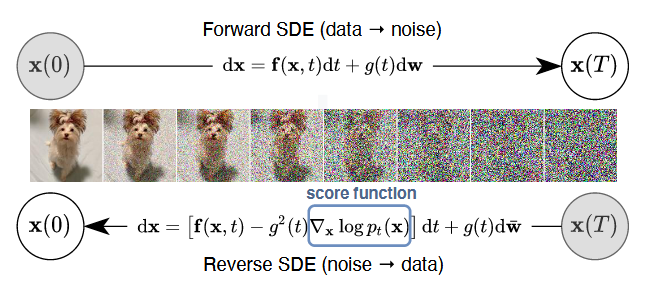
\includegraphics[width=0.8\textwidth]{./pics/score_based.png} % 图片路径和大小
    \caption{score-based generative model}
\end{figure}


The most difficult question on how to obtian $\nabla_x \log p(x)$ because it solves FPK equation.

\textbf{Explicit Score Matching}
Suppose we have a set of samples $x_1, x_2, \cdots, x_n$ from the data distribution $p_{data}(x)$. 
A classical way is to consider the kernel density estimation $q(x)$ of $p(x)$:
\begin{equation}
    q(x) = \frac{1}{n}\sum_{i=1}^n K(x-x_i)
\end{equation}
where $K(x)$ is the kernel function. Since $q(x)$ is an approximation to $p_{data}$. 
We can define a loss function to train a network:
\begin{equation}
    \begin{aligned}
        \mathcal{L}_\theta =& \mathbf{E}_{x\sim p(x)} \left[\left\|s_\theta(x) - \nabla_x \log p(x)\right\|^2\right]\\
        \approx& \mathbf{E}_{x\sim q(x)} \left[\left\|s_\theta(x) - \nabla_x \log q(x)\right\|^2\right]\\
        =& \int \left\|s_\theta (x) - \nabla_x \log q(x)\right\|^2 q(x) dx\\
        \approx & \frac{1}{n}\sum_{i=1}^n \int \left\|s_\theta (x) - \nabla_x \log q(x)\right\|^2 K(x-x_i) dx
    \end{aligned}
\end{equation}
However, when the number of samples is limited, the estimation $\nabla_x \log q(x)$ is not accurate.

\textbf{Implicit Score Matching}

\textbf{Denoising Score Matching}
Normally we can define the loss function as follows:
\begin{equation}
    \begin{aligned}
        L_\theta & = \frac{1}{T}\int_0^T\lambda(t)\underset{x_0\sim p_{data}}{E}\left[\underset{x_t\sim p_{t|0}(x_t|x_0)}{E}\left[\|s_\theta(x_t, t)-\nabla_{x_t}\log p_t(x_t)\|^2\right]\right]dt\\
        &=\underset{t\sim U(0, T)}{E}\left[\lambda(t)\underset{x_0\sim p_{data}}{E}\left[\underset{x_t\sim p_{t|0}(x_t|x_0)}{E}\left[\|s_\theta(x_t, t)-\nabla_{x_t}\log p_t(x_t)\|^2\right]\right]\right]
    \end{aligned}
\end{equation}
It should be clearified that $p_{t|0}(x_t|x_0)=p(X_t=x_t|X_0=x_0)$. So $$p_t(x_t)=\int p_{t|0}(x_t|x_0)p_0(x_0)dx_0=E_{x_0\sim p_{data}}\left[p_{t|0}(x_t|x_0)\right]$$
where $p_{t}(x)=p\left(X_{t}=x\right)$, $p_{t | 0}(x | y)=p\left(X_{t}=x | X_{0}=y\right)$. Then

\begin{equation}
    \begin{aligned}
    \nabla \log p_{t}(x) & =\frac{1}{p_{t}(x)} \nabla p_{t}(x) . \\
    & =\frac{1}{p_{t}(x)} \nabla \int p_{t | 0}(x | y) p_{0}(y) d y \\
    & =\frac{1}{p_{t}(x)} \int \nabla p_{t | 0}(x | y) p_{0}(y) d y \\
    & =\frac{1}{p_{t}(x)} \int \frac{\nabla p_{t | 0}(x | y)}{p_{t | 0}(x | y)} p_{0}(y) \cdot p_{t | 0}(x | y) d y \\
    & =\int \nabla_{x} \log \left(p_{t | 0}(x | y)\right) \cdot p_{0 | t}(y | x) d y \\
    & =\underset{y\sim p_{0|t}(y|x)}{E}\left[\nabla_{x} \log \left(p_{t | 0}(x | y)\right)\right]
    \end{aligned}
\end{equation}

Where we have used the following lemma:
\begin{lemma}
    \begin{equation}
        \underset{x_0\sim p_0}{E}\left[\underset{x_t\sim p_{t|0}(\cdot|x_0)}{E}\left[\underset{x'_0\sim p_{0|t}(\cdot|x_t)}{E}\left[f(x_t, x'_0)\right]\right]\right]=\underset{x_0\sim p_0}{E}\left[\underset{x_t\sim p_{t|0}(\cdot|x_0)}{E}\left[f(x_t, x_0)\right]\right]
    \end{equation}
\end{lemma}
\begin{proof}
    Easy to prove.
\end{proof}
Then we can rewrite the loss function as:
\begin{equation}
    \begin{aligned}
        L_{\theta}&=\underset{t\sim U(0,T)}{E}\left[\lambda(t) \underset{x_{0}\sim p_{data}}{E}\left[\underset{x_{t}\sim p_{t|0}(x_t|x_0)}{E}\left[\left\|S_{\theta}\left(x_{t}, t\right)-\nabla _{x_t}\log p_{t}\left(x_{t}\right)\right\|^{2}\right]\right.\right.\\ 
        &\leqslant \underset{t\sim U(0,T)}{E}\left[\lambda(t) \underset{x_{0}\sim p_{data}}{E}\left[\underset{x_{t}\sim p_{t|0}(x_t|x_0)}{E}\left[\underset{y\sim p_{data}}{E}\left[\left\|S_{\theta}\left(x_{t}, t\right)-\nabla_{x_{t}} \log \left(p_{t|0}(x_t | y)\right)\right\|^{2}\right]\right]\right]\right] \\
        &=\underset{t\sim U(0, T)}{E}\left[\lambda(t) \underset{x_{0}\sim p_{data}}{E}\left[\underset{x_{t}\sim p_{t|0}(x_t|x_0)}{E}\left[\| S_{\theta}\left(x_{t}, t\right)-\nabla_{x_{t}} \log \left(p_{t|0}\left(x_{t} | x_{0}\right) \|^{2}\right]\right]\right]\right.
    \end{aligned}
\end{equation}


Since  $p_{t|0}\left(x_{t} | x_{0}\right)=p\left(X_{t}=x_{t} | X_{0}=x_{0}\right)$  has been discussed:

$$p_{t | 0}\left(x_{t} | x_{0}\right) \sim N\left(x_{t} ; E\left[X_{t}=x_t | X_{0}=x_{0}\right], \operatorname{Var}\left(X_{t}=x_t | X_{0}=x_{0}\right)\right) .$$

Then by theorem \ref{thm1}, x can be written as $x=e(t, X_0)+\sqrt{V(t)}\xi$, where $\xi\sim N(0, 1)$, then the score function is:
\begin{equation}
    \frac{\partial}{\partial x} \log p_{t | 0}\left(x | x_{0}\right)=-\frac{x-E_{t | 0}\left[x | x_{0}\right]}{\operatorname{Var}_{t | 0}\left(x | x_{0}\right)}=-\frac{x-e(t, X_0)}{V(t)}\sim -N\left(0, \frac{1}{V(t)}\right)
\end{equation}
So
\begin{equation}
\begin{aligned}
    L_\theta=&\underset{t\sim U(0,T)}{E}\left[\lambda (t)\underset{x_0\sim p_{data}}{E}\left[\underset{\xi\sim N(0, 1)}{E}\left[\left\|s_\theta\left(\sqrt{V(t)}\xi+e(t, X_0), t\right) + \frac{\xi}{\sqrt{V(t)}}\right\|^2\right]\right]\right]\\
    =&\underset{t\sim U(0,T)}{E}\left[\lambda (t)\underset{x_0\sim p_{data}}{E}\left[\frac{1}{V(t)}\underset{\xi\sim N(0, 1)}{E}\left[\left\|\xi_\theta\left(\sqrt{V(t)}\xi+e(t, X_0), t\right)-\xi\right\|^2\right]\right]\right]
\end{aligned}    
\end{equation}
where $\xi_\theta = -\sqrt{V(t)}s_\theta$ is called denoising network.

\subsubsection{With labels}

\paragraph{With Classifier Guidance}
Though we can produce pictures by sampling from normal distribution, we still cannot control what we will generate. What we want to do is something like:
"Give me the pictures of number 6", then the model can sample from the normal distribution and do the denoising to generate pics of 6. 

Usually, we can do something like: train a model for every class label. This do make the model smaller, but increases number of models. 
Think about it, when the label is TEXT, it is impossiable to train a model for each sentences. 

So, the initial distribution is $p_0(x|y)$ given the label y. Similarly, we will convert the data distribution $p_{data}(x|y)$ to final distribution, normal distribution expected.
Then we SDE becomes: $X_t \sim p_t(x|y)$


\begin{equation}
    \begin{aligned}
    & p_{t}(x \mid y)=p\left(X_{t}=x \mid y\right)=\frac{p\left(y \mid X_{t}=x\right) p\left(X_{t}=x\right)}{p(y)} \\
    \Rightarrow & \log \left(p_{t}(x \mid y)\right)=\log \left(p\left(y \mid X_{t}=x\right)\right)+\log \left(p\left(X_{t}=x\right)\right)-\log (p(y)) \\
    \Rightarrow & \nabla_{x} \log \left(p_{t}(x \mid y)\right)=\nabla_{x} \log \left(p\left(y \mid X_{t}=x\right)\right)+\nabla_{x} \log \left(p\left(X_{t}=x\right)\right)
    \end{aligned}
\end{equation}
    
    
We have finished training  $\nabla_{x} \log \left(p\left(X_{t}=x\right)\right)$  in sampling. Then we need to estimate  $\nabla_{x} \log \left(p\left(y \mid X_{t}=x\right)\right)$. This is the conditional protability, we end up with a sharp factor s: $p^{\prime}\left(y \mid X_{t}=x\right)$ , then:
\begin{equation}
    \nabla_{x} \log \left(p_{t}(x \mid y)\right)=S \nabla_{x} \log \left(p\left(y \mid x_{t}=x\right)\right)+\nabla_{x} \log \left(p\left(x_{t}=x\right)\right)
\end{equation}
Note  $\omega_{\theta}(y \mid x, t)$  to learn  $s \nabla_{x} \log \left(p\left(y \mid X_{t}=x\right)\right)$ 

\paragraph{Classifier Guidance Free}
\begin{equation}
    \begin{aligned}
        &\gamma \nabla_{x} \log \left(p\left(y \mid X_{t}=x\right)\right)\\
         =& \gamma\left(\nabla_x \log \left(p(X_t=x|y)\right) - \nabla_x \log \left(p_t(x)\right)\right)
    \end{aligned}
\end{equation}
Then 
\begin{equation}
    \begin{aligned}
        &\nabla_{x} \log_\gamma \left(p_{t}(x \mid y)\right)\\
        =&(1-\gamma)\nabla_x \log \left(p_t(x)\right) + \gamma\nabla_x \log \left(p(X_t=x|y)\right)
    \end{aligned}
\end{equation}
Hence we only need one conditional denoising network, and using null condition to represent the unconditional model.

\subsection{Flow Matching}
We have discussed the FPK Equation in 'learnsde'. 
\begin{theorem}[Fokken-Planck-Kolmogorov equation]
    The density function $p(x, t)$ of $X_t$ s.t. 
    \begin{equation}
        dX_t = f(X_t, t)dt + G(X_t,t)dW_t
    \end{equation}
    solves the PDE:
    \begin{equation}
        \frac{\partial p(x, t)}{\partial t}=-\sum_{i} \frac{\partial}{\partial x_{i}}\left[f_{i}(x, t) p(x, t)\right]+\frac{1}{2} \sum_{i, j} \frac{\partial^{2}}{\partial x_{i} \partial x_{j}}\left[\left(G Q G^{\top}\right)_{i j} p(x, t)\right]
    \end{equation}
    The PDE is called FPK equation / forwand Kolmogorov equation.
\end{theorem}
It can be rewritten as:
\begin{equation}
    \begin{aligned}
        \frac{\partial p(x, t)}{\partial t} &= -\nabla\cdot\left[f(x, t) p(x, t)\right]+\frac{1}{2} \nabla^2\cdot\left[\left(G Q G^{\top}\right) p(x, t)\right] \\
        &=-\nabla\cdot\left[f(x, t) p(x, t)-\frac{1}{2} \nabla\cdot\left[\left(G Q G^{\top}\right) p(x, t)\right]\right]
    \end{aligned}
\end{equation}
Here, if we only consider $G(X_t, t)=g(t)$, then we notice that $M=GQG^T$ is independent of $X_t$, so we can write:
\begin{equation}
    \begin{aligned}
        \frac{\partial p(x, t)}{\partial t} &= -\nabla\cdot\left(fp-\frac{1}{2}\nabla\cdot (Mp)\right)\\
        &=-\nabla\cdot\left(fp-\frac{1}{2}M\nabla p\right)\\
        &=-\nabla\cdot\left[\left(f-\frac{1}{2}M\frac{\nabla p}{p}\right)p\right]\\
        &=-\nabla\cdot\left[\left(f-\frac{1}{2}M\nabla\log p\right)p\right]
    \end{aligned}
\end{equation}
So we find out that if we have an ODE s.t. $dZ_t=F(Z_t, t)dt$ with $Z_0 \sim p_0$, instead of a SDE, then by FPK equation, the density $p(z, t)$ satisfies:
\begin{equation}
    \frac{\partial p(z, t)}{\partial t}=-\nabla\cdot\left(F(z, t)p(z, t)\right)
\end{equation}
So if we set $F(z, t)=f(z, t) - \frac{1}{2}M(t)\nabla\log p(z, t)$, then $p(z, t)$ is exactly like the density $p(x, t)$ of $X_t$ in SDE. 
So theoretically, we can do the diffusion like reverse ode!

This is the topic discussed in 'Probability Flow'.

Define a flow $\phi: \mathcal{R}^d\times [0, 1]\rightarrow \mathcal{R}^d$ is a flow generated by a vector field $v: \mathcal{R}^d \times [0, 1]\rightarrow \mathcal{R}^d$ i.e.
\begin{equation}\left\{
    \begin{aligned}
        \frac{\partial \phi(x, t)}{\partial t} &= v(\phi(x, t), t)\\
        \phi(0, x)&=x
    \end{aligned}\right.
\end{equation}
The flow means that under the vector field $v$, if the initial point is $x$, then the flow push the point after time $t$ to $\phi(x, t)$. That is $\phi$ gives the evolution trajectory of $x$ under the vector field $v$.
So normally, we can consider the flow $\phi(x, t)$ as $X_t$ in SDE:
\begin{equation}
    dX_t = v(X_t, t)dt + 0dW_t
\end{equation}
with $X_0=x$. It turns out that it is actually an ODE, a SDE without diffusion term. Similar to SDE, if $X_0=x\sim p_0(x)$, we have the probability density $p(x, t)$ satisfies FPK equation:
\begin{equation}
    \frac{\partial p(x, t)}{\partial t}=-\nabla\cdot\left(v(x, t)p(x, t)\right)
\end{equation}
which is a special case of FPK equation, called \textbf{Continuity Equation}. So, typically, we can solution to an ODE is a flow.



So the objective of Flow Matching Model can be described as: Let $p_t(x)$ be the density with initial $p_0(x)$, which is designed to be a simple distribution, like normal distribution. 
So let $p_1(x)$ be the approximation equal in distribution to$ p_{data}$. Then we need to design a flow to match the flow s.t. $p_1$ can properly approximate $p_{data}$.

\subsection{Variational Auto-Encoder}
Variational Autoencoders aim to learn both an encoder and a decoder to map input data to values in  a continuous latent space.
In these models, the embedding can be interpreted as a latent variable in a probabilistic  generative model, and a probabilistic decoder can be formulated by a parameterized likelihood function. In addition,  the data x is assumed to be generated by some unobserved latent variable z.

\begin{figure}[H]
    \centering
    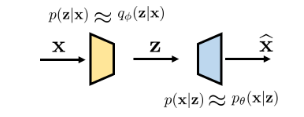
\includegraphics[width=0.5\textwidth]{./pics/VAE.png} % 图片路径和大小
    \caption{VAE block}
\end{figure}
where $q_{\phi}(\mathbf{z} \mid \mathbf{x})$ is the proxy for  $p(\mathbf{z} \mid \mathbf{x})$, which is also the distribution associated with the encoder.  
And $p_{\boldsymbol{\theta}}(\mathbf{x} \mid \mathbf{z})$ is the proxy for  $p(\mathbf{x} \mid \mathbf{z})$ , which is also the distribution associated with the decoder. 
Like the encoder, the decoder can be parameterized by a deep neural network. 

If we treat $\phi$ and $\theta$ as optimization variables, then we need an objective function (or the loss function) so that we can optimize $\phi$ and $\theta$ through training samples.
\begin{definition}[Evidence Lower Bound]
    The Evidence Lower Bound (ELBO) is defined as:
    \begin{equation}
        \operatorname{ELBO}(x) = \mathbf{E}_{q_\phi(z|x)}\left[\log \frac{p(x, z)}{q_\phi(z|x)}\right]
    \end{equation}
\end{definition}
\begin{remark}
    The ELBO is a lower bound of the log-likelihood of the data. It is used to estimate $\log p(x)$.
    \begin{equation}
        \begin{aligned}
            \log p(x) &= \log \int p(x, z) dz\\
            & = \log \int \frac{p(x, z)}{q_\phi(z|x)} \cdot q_\phi(z|x) dz\\
            & \geq \mathbf{E}_{q_\phi(z|x)}\left[\log \frac{p(x, z)}{q_\phi(z|x)}\right] = \operatorname{ELBO}(x)
        \end{aligned}
    \end{equation}
\end{remark}
\begin{theorem}[Decomposition of Log-likelihood]
    We have 
    \begin{equation}
        \log p(x) =\operatorname{ELBO}(x) + \operatorname{KL}(q_\phi(z|x)||p(z|x))
    \end{equation}
    then we can minimize the gap between $\log p(x)$ and ELBO, and the equality hold if and only if $q_\phi(z|x)=p(z|x)$.

    Since $p(z|x)$ is a delta function, 
\end{theorem}
\begin{proof}
    \begin{equation}
        \begin{aligned}
            \log p(x) & = \log p(x)\int q_\phi(z|x)dz\\
            &=\mathbf{E}_{q_\phi(z|x)}\left[\log p(x)\right]\\
            & = \mathbf{E}_{q_\phi(z|x)}\left[\log \left(\frac{p(x, z)}{p(z|x)}\frac{q_\phi(z|x)}{q_\phi(z|x)}\right)\right]\\
            & =\operatorname{ELBO}(x) + \operatorname{KL}(q_\phi(z|x)||p(z|x))
        \end{aligned}
    \end{equation}
\end{proof}

\begin{theorem}
    Also, we can rewrite the ELBO as:
    \begin{equation}
        \begin{aligned}
            \operatorname{ELBO}(x) &= \mathbf{E}_{q_\phi(z|x)}\left[\log p(x|z)+\log p(z)-\log q_\phi(z|x)\right]\\
            &= \mathbf{E}_{q_\phi(z|x)}\left[\log p(x|z)\right] - \operatorname{KL}(q_\phi(z|x)||p(z))\\
            &= \mathbf{E}_{q_\phi(z|x)}\left[\log p_\theta(x|z)\right] - \operatorname{KL}(q_\phi(z|x)||p(z))
        \end{aligned}
    \end{equation}
    where the first term determines how good the decoder is, maxmizing the likelihood of observing the image, 
    and the letter describes how good the encoder is, minimizing the distance between two distributions.
\end{theorem}

\begin{definition}[The objective of VAE]
    The optimiztion objective of VAE is to maxmize the ELBO:
    \begin{equation}
        (\phi, \theta) = \operatorname{argmax}_{\phi, \theta} \sum_{x\in X} \operatorname{ELBO(x)}
    \end{equation}
    where $X$ is the training set.
\end{definition}
The DDPM can be conceptualized as a hierarchical Markovian VAE with a fixed encoder. Specifically, DDPM's  forward process functions as the encoder.
The DDPM’s reverse process, on the other hand, corresponds to the decoder, which is shared across multiple  decoding steps. The latent variables within the decoder are all the same size as the sample data.